\documentclass[10pt]{beamer}

\usepackage[utf8]{inputenc}
\usepackage{pgfpages}
\usepackage{dirtree}
\setbeamertemplate{note page}[plain]
\AtEndNote{\vfill \begin{center} mm:hh \end{center}}
\newcommand{\notedir}[1] {
  \note{\dirtree{#1}}}
\usepackage{tcolorbox}
\usepackage{tikz}
\usepackage{tikz-3dplot}
\usetikzlibrary{intersections,calc,,angles,quotes,through}
\usepackage{amsmath}
\usepackage{graphicx}
\usepackage{cases}
\def \heart {\textcolor{blue}{$\heartsuit$} }
\def \C {\mathcal{C}}
\def \orthog {\underline{\perp}}
\def\arcos{\operatorname{arcos}}
\def \deg {^{\circ}}

\newcommand{\vect}[1] {
  \overrightarrow{#1}}

\tcbset{%
	basic/.style={colframe=black,
		      colback=white,
		      top= 0mm,
		      bottom = 2mm,
		      boxsep=0mm
		      }
}
\tikzset{
    invisible/.style={opacity=0},
    visible on/.style={alt={#1{}{invisible}}},
    alt/.code args={<#1>#2#3}{%
      \alt<#1>{\pgfkeysalso{#2}}{\pgfkeysalso{#3}} % \pgfkeysalso doesn't change the path
    },
  }

    
\begin{document}  
    \beamertemplatenavigationsymbolsempty
    \setlength{\abovedisplayskip}{0pt}
    \setlength{\belowdisplayskip}{0pt}
    
    \frame{\frametitle{Angles égaux.}
	
	\begin{columns}[t]
	 \column{.25\textwidth}\centering
	 \underline{Opposés} \\
	 \underline{par le sommet.}
	 \begin{figure}
				  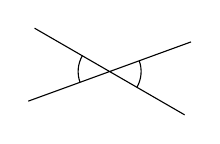
\begin{tikzpicture}[scale=0.55]
			          %projection ($(X)!(B')!(B)$)
			          %nommer chemin 'name path
			          %intersections \path [name intersections={of=d and gb,name=G}];
			          %intersection \path [name intersections={of=d and gb,by=G}];
			          %animation  \draw[visible on=<1>] 
				  %           \draw[visible on=<{2,4}>]
				  %angle arc[radius = 6mm, start angle= 180, end angle= 225] node [below left,pos=0.3]{$\alpha$}
				  %angle \pic [draw,"$\alpha$", angle eccentricity=1.5] {angle = A'--A--B};
				  %perpendiculaire ($(A')!3cm!-90:(A)$)
				  %cercle par point \node [draw] at (A) [circle through=(B)] {};
				  \coordinate(A) at (200:2);
				  \coordinate(B) at (20:2);
				  \coordinate(C) at (150:2);
				  \coordinate(D) at (-30:2);
				  \coordinate(O) at (0,0);

				  \draw (A) -- (B) (C) -- (D);
				  \pic [draw, angle eccentricity=1.5, angle radius=4mm] {angle = C--O--A};
				  \pic [draw, angle eccentricity=1.5, angle radius=4mm] {angle = D--O--B};
				  \end{tikzpicture}
				  \end{figure}
				
	 \column{.25\textwidth}\centering
	 \underline{À cotés} \\
	 \underline{perpendiculaires.}
	 \begin{figure}
				  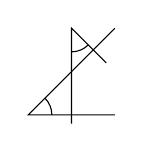
\begin{tikzpicture}[scale=0.55]
			          %projection ($(X)!(B')!(B)$)
			          %nommer chemin 'name path
			          %intersections \path [name intersections={of=d and gb,name=G}];
			          %intersection \path [name intersections={of=d and gb,by=G}];
			          %animation  \draw[visible on=<1>] 
				  %           \draw[visible on=<{2,4}>]
				  %angle arc[radius = 6mm, start angle= 180, end angle= 225] node [below left,pos=0.3]{$\alpha$}
				  %angle \pic [draw,"$\alpha$", angle eccentricity=1.5] {angle = A'--A--B};
				  %perpendiculaire ($(A')!3cm!-90:(A)$)
				  %cercle par point \node [draw] at (A) [circle through=(B)] {};
				  \coordinate(O) at (0,0);
				  \coordinate(A) at (2,0);
				  \coordinate(B) at (2,2);
				  \draw (A) -- (O) -- (B);
				  
				  \coordinate(C) at (1,2);
				  \coordinate(D) at (1,-0.2);
				  \coordinate(E) at (1.8,1.2);
				  \draw (D)--(C)--(E);
				  
				  \pic [draw, angle eccentricity=1.5, angle radius=3mm] {angle = A--O--B};
				  \pic [draw, angle eccentricity=1.5, angle radius=3mm] {angle = D--C--E};
				  \end{tikzpicture}
				  \end{figure}
	\column{.25\textwidth}\centering
	 \underline{À côtés} \\
	 \underline{parallèles.}
	 \begin{figure}
				  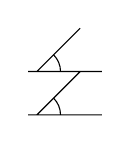
\begin{tikzpicture}[scale=0.55]
			          %projection ($(X)!(B')!(B)$)
			          %nommer chemin 'name path
			          %intersections \path [name intersections={of=d and gb,name=G}];
			          %intersection \path [name intersections={of=d and gb,by=G}];
			          %animation  \draw[visible on=<1>] 
				  %           \draw[visible on=<{2,4}>]
				  %angle arc[radius = 6mm, start angle= 180, end angle= 225] node [below left,pos=0.3]{$\alpha$}
				  %angle \pic [draw,"$\alpha$", angle eccentricity=1.5] {angle = A'--A--B};
				  %perpendiculaire ($(A')!3cm!-90:(A)$)
				  %cercle par point \node [draw] at (A) [circle through=(B)] {};
				  \coordinate(O) at (0,0);
				  \coordinate(A) at (-0.2,0);
				  \coordinate(B) at (1.5,0);
				  \coordinate(C) at (-0.2,1);
				  \coordinate(D) at (1,1);
				  \coordinate(E) at (1.5,1);
				  \coordinate(F) at (1,2);
				  \coordinate(G) at (0,1);
				  
				  \draw(A) -- (B) (C) -- (E) (O) -- (D) (G) -- (F);
				  
				  \pic [draw, angle eccentricity=1.5, angle radius=3mm] {angle = B--O--D};
				  \pic [draw, angle eccentricity=1.5, angle radius=3mm] {angle = D--G--F};
				  \end{tikzpicture}
				  \end{figure}
				  
	\column{.25\textwidth}\centering
	 \underline{Alternes -} \\
	 \underline{internes.}
	 \begin{figure}
				  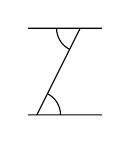
\begin{tikzpicture}[scale=0.55]
			          %projection ($(X)!(B')!(B)$)
			          %nommer chemin 'name path
			          %intersections \path [name intersections={of=d and gb,name=G}];
			          %intersection \path [name intersections={of=d and gb,by=G}];
			          %animation  \draw[visible on=<1>] 
				  %           \draw[visible on=<{2,4}>]
				  %angle arc[radius = 6mm, start angle= 180, end angle= 225] node [below left,pos=0.3]{$\alpha$}
				  %angle \pic [draw,"$\alpha$", angle eccentricity=1.5] {angle = A'--A--B};
				  %perpendiculaire ($(A')!3cm!-90:(A)$)
				  %cercle par point \node [draw] at (A) [circle through=(B)] {};
				  \coordinate(O) at (0,0);
				  \coordinate(A) at (-0.2,0);
				  \coordinate(B) at (1.5,0);
				  \coordinate(C) at (-0.2,2);
				  \coordinate(D) at (1,2);
				  \coordinate(E) at (1.5,2);
				  
				  \draw(A) -- (B) (C) -- (E) (O) -- (D);
				  
				  \pic [draw, angle eccentricity=1.5, angle radius=3mm] {angle = B--O--D};
				  \pic [draw, angle eccentricity=1.5, angle radius=3mm] {angle = C--D--O};
				  \end{tikzpicture}
				  \end{figure}
	\end{columns}
	
}
    
    \frame{
    
	  \frametitle{Triangles.}
	  \underline{Droites remarquables.}
	  \bigskip
	  
	  \begin{figure}[h]
				  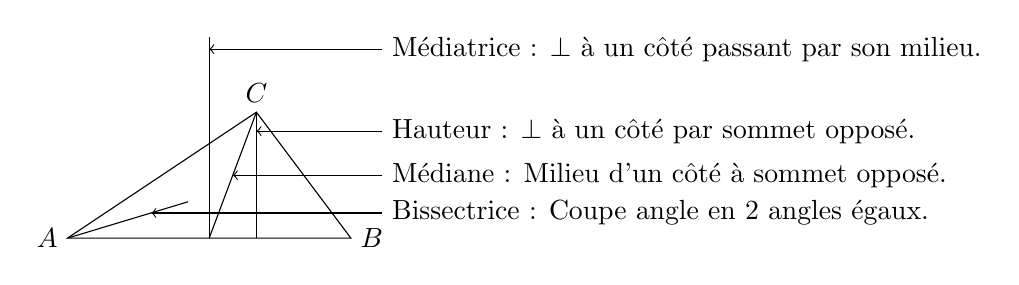
\begin{tikzpicture}[scale=0.8]
			          %projection ($(X)!(B')!(B)$)
			          %nommer chemin 'name path
			          %intersections \path [name intersections={of=d and gb,name=G}];
			          %intersection \path [name intersections={of=d and gb,by=G}];
			          %animation  \draw[visible on=<1>] 
				  %           \draw[visible on=<{2,4}>]
				  %angle arc[radius = 6mm, start angle= 180, end angle= 225] node [below left,pos=0.3]{$\alpha$}
				  %angle \pic [draw,"$\alpha$", angle eccentricity=1.5] {angle = A'--A--B};
				  %perpendiculaire ($(A')!3cm!-90:(A)$)
				  %cercle par point \node [draw] at (A) [circle through=(B)] {};
				  \coordinate[label=left:$A$](A) at (-3,0);
				  \coordinate[label=right:$B$](B) at (1.5,0);
				  \coordinate[label=above:$C$](C) at (0,2);
				  \coordinate[label=right:Médiatrice : $\bot$ à un côté passant par son milieu.](Mediatrice) at (2,3);
				  \coordinate[label=right:Médiane : Milieu d'un côté à sommet opposé.](Mediane) at (2,1);
				  \coordinate[label=right:Hauteur : $\bot$ à un côté par sommet opposé.](Hauteur) at (2,1.7);
				  \coordinate[label=right:Bissectrice : Coupe angle en 2 angles égaux.](Bissectrice) at (2,0.4);
				  \coordinate (M) at ($(A)!.5!(B)$);
				  \draw (A) -- (B) -- (C) -- cycle;
				  \draw (M) -- (C);
				  \draw (M) -- +(0,3) coordinate(top_mediatrice) -- +(0,3.2);
				  \draw (0,0) -- (C);
				  \draw (A) -- +(16.8:2);
				  \draw[->] (Mediane) -- ($(M)!.5!(C)$);
				  \draw[->] (Mediatrice) -- (top_mediatrice);
				  \draw[->] (Hauteur) -- +(-2,0);
				  \draw[->] (Bissectrice) -- +(-3.67,0);
				  \end{tikzpicture}
				  \end{figure}
	  \bigskip
	  \begin{center}
	  \begin{tabular}{l l l}
	   Hauteurs & concourantes en & orthocentre. \\ 
	   Médianes & concourantes en & centre de gravité. \\
	   Médiatrices & concourantes en & centre du cercle circonscrit. \\
	   Bissectrices & concourantes en & centre du cercle inscrit. \\
	  \end{tabular}
	  \end{center}
	  

	\notedir{%
	.1 Droites remarquables.
	.2 Définitions..
	.2 Points remarquables..
	}
	  
	
    }

    \frame{ \renewcommand{\arraystretch}{2}
	  \frametitle{Triangles.}
	  
	  \begin{tabular}{c|c|c}
				    & \underline{Isométriques} & \underline{Semblables}\\[1em] \hline 
	  \parbox{2.2cm}{Conditions\\ (une à monter)} & \begin{minipage}{4cm}\bigskip
	                               \begin{itemize}
	                               \item 1 côté compris entre\\ 2 angles égaux.
	                               \item 1 angle compris entre\\ 2 côtés égaux.
	                               \item 3 côtés égaux.
	                              \end{itemize}
	                              \end{minipage}
				      &\begin{minipage}{4.2cm}\bigskip
	                               \begin{itemize}
	                               \item 2 angles égaux.\\[1.5em] 
	                               \item 1 angle compris entre\\ 2 côtés proportionnels.
	                               \item 3 côtés proportionnels.\\
	                              \end{itemize}
	                              \end{minipage} \\[5em] \hline
	  
	   
	\parbox{2.2cm}{Implications}& \parbox{4.2cm}{\bigskip \centering 3 côtés égaux et\\ 3 angles égaux.}&\parbox{4.2cm}{\bigskip \centering 3 côtés proportionnels et\\ 3 angles égaux.} \\ 				
	  
	  \end{tabular}
	  \notedir{%
	  .1 Triangles isométriques et semblables.
	  .2 Isométriques.
	  .3 Conditions.
	  .4 Côté de même longueur compris entre 2 angles de mêmes mesures..
	  .4 Angle de même mesure compris entre 2 côtés de mêmes longueurs..
	  .4 Longueurs de leurs côtés sont 2 à 2 égales..
	  .3 Implications.
	  .4 Longueurs des côtés 2 à 2 égales..
	  .4 Angles 2 à 2 égaux..
	  .2 Semblables.
	  .3 Conditions.
	  .4 Côtés proportionnels..
	  .4 2 angles de l'un égaux à 2 angles de l'autre..
	  .4 2 côtés de l'un proportionnels à 2 côtés de l'autre et angle entre les 2 côtés égaux.
	  .3 Implications.
	  .4 Côtés proportionnels et angles 2 à 2 égaux..
	  }
    }
\frame{ \frametitle{Triangles.}
	\underline{Pythagore généralisé.}
	\vspace{-3mm}
	\begin{figure}
				  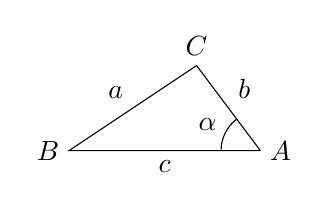
\begin{tikzpicture}[scale=0.54]
			          %projection ($(X)!(B')!(B)$)
			          %nommer chemin 'name path
			          %intersections \path [name intersections={of=d and gb,name=G}];
			          %intersection \path [name intersections={of=d and gb,by=G}];
			          %animation  \draw[visible on=<1>] 
				  %           \draw[visible on=<{2,4}>]
				  %angle arc[radius = 6mm, start angle= 180, end angle= 225] node [below left,pos=0.3]{$\alpha$}
				  %angle \pic [draw,"$\alpha$", angle eccentricity=1.5] {angle = A'--A--B};
				  %perpendiculaire ($(A')!3cm!-90:(A)$)
				  %cercle par point \node [draw] at (A) [circle through=(B)] {};
				  \coordinate[label=left:$B$](B) at (-3,0);
				  \coordinate[label=right:$A$](A) at (1.5,0);
				  \coordinate[label=above:$C$](C) at (0,2);
				  \draw (A) -- node[below]{$c$}  (B) -- node[above left]{$a$} (C) -- node[above right]{$b$} (A);
				  \pic [draw,"$\alpha$", angle eccentricity=1.5] {angle = C--A--B};
				  \end{tikzpicture}
				  \end{figure}
				  $$a^2 = b^2 + c^2 -2bc\operatorname{cos}(\alpha)$$
				\medskip
                                \underline{Médiane issue de l'angle droit d'un triangle rectangle.} \\
                                $\Delta ABC$ rectangle et $M$ milieu $[BC]$.
				  \begin{figure}
				  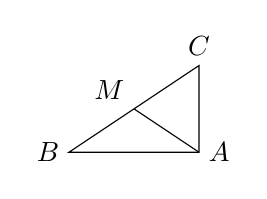
\begin{tikzpicture}[scale=0.55]
			          %projection ($(X)!(B')!(B)$)
			          %nommer chemin 'name path
			          %intersections \path [name intersections={of=d and gb,name=G}];
			          %intersection \path [name intersections={of=d and gb,by=G}];
			          %animation  \draw[visible on=<1>] 
				  %           \draw[visible on=<{2,4}>]
				  %angle arc[radius = 6mm, start angle= 180, end angle= 225] node [below left,pos=0.3]{$\alpha$}
				  %angle \pic [draw,"$\alpha$", angle eccentricity=1.5] {angle = A'--A--B};
				  %perpendiculaire ($(A')!3cm!-90:(A)$)
				  %cercle par point \node [draw] at (A) [circle through=(B)] {};
				  \coordinate[label=left:$B$](B) at (-3,0);
				  \coordinate[label=right:$A$](A) at (0,0);
				  \coordinate[label=above:$C$](C) at (0,2);
				  \coordinate[label=above left:$M$](M) at ($(B)!.5!(C)$);
				  \draw (A) -- (B) -- (C) -- cycle;
				  \draw (A) -- (M);
				  \end{tikzpicture}
				  \end{figure}
				  $$|AM| = |BM| = |CM| $$
				  
		\notedir{%
		.1 Relations de longueurs.
		.2 Pythagore généralisé..
		.3 Formule valable pour n'importe quel côté.~Pas seulement pour le côté le plus long..
		.3 Énoncé en français aide à connaître formule..
		.2 Médiane issue de l'angle droit d'un triangle rectangle.
		.3 Car $\Delta$ rect.~inscriptible dans demi-cercle de centre $M$.. 
		.4 $A,B,C$ sont à équidistance de $M$..
		}
}

\frame{ \frametitle{Triangles.}
	\underline{Relation des sinus.}
	\begin{figure}
				  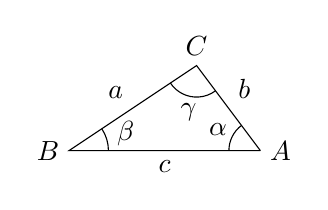
\begin{tikzpicture}[scale=0.54]
			          %projection ($(X)!(B')!(B)$)
			          %nommer chemin 'name path
			          %intersections \path [name intersections={of=d and gb,name=G}];
			          %intersection \path [name intersections={of=d and gb,by=G}];
			          %animation  \draw[visible on=<1>] 
				  %           \draw[visible on=<{2,4}>]
				  %angle arc[radius = 6mm, start angle= 180, end angle= 225] node [below left,pos=0.3]{$\alpha$}
				  %angle \pic [draw,"$\alpha$", angle eccentricity=1.5] {angle = A'--A--B};
				  %perpendiculaire ($(A')!3cm!-90:(A)$)
				  %cercle par point \node [draw] at (A) [circle through=(B)] {};
				  \coordinate[label=left:$B$](B) at (-3,0);
				  \coordinate[label=right:$A$](A) at (1.5,0);
				  \coordinate[label=above:$C$](C) at (0,2);
				  \draw (A) -- node[below]{$c$}  (B) -- node[above left]{$a$} (C) -- node[above right]{$b$} (A);
				  \pic [draw,"$\alpha$", angle eccentricity=1.5, angle radius=4mm] {angle = C--A--B};
				  \pic [draw,"$\beta$", angle eccentricity=1.5] {angle = A--B--C};
				  \pic [draw,"$\gamma$", angle eccentricity=1.5, angle radius=4mm] {angle = B--C--A};
				  \end{tikzpicture}
				  \end{figure}
				  $$\frac{a}{\operatorname{sin}\alpha} = \frac{b}{\operatorname{sin}\beta} = \frac{c}{\operatorname{sin}\gamma}$$
				 \medskip
				
		\notedir{%
		.1 Relations de longueurs.
		.2 Pythagore généralisé..
		.3 Formule valable pour n'importe quel côté.~Pas seulement pour le côté le plus long..
		.3 Énoncé en français aide à connaître formule..
		.2 Médiane issue de l'angle droit d'un triangle rectangle.
		.3 Car $\Delta$ rect.~inscriptible dans demi-cercle de centre $M$.. 
		.4 $A,B,C$ sont à équidistance de $M$..
		}
}

\frame{ \frametitle{Cercles.}
\underline{Angles particuliers.} \\ \bigskip
				  \begin{figure}
				  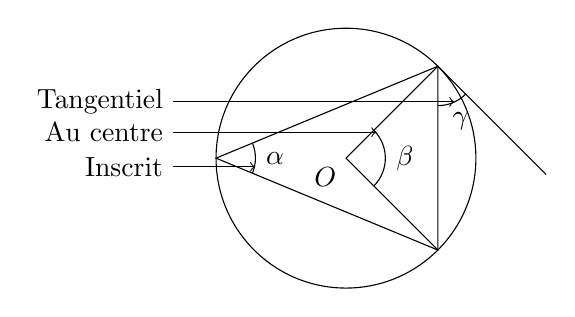
\begin{tikzpicture}[scale=0.55]
			          %projection ($(X)!(B')!(B)$)
			          %nommer chemin 'name path
			          %intersections \path [name intersections={of=d and gb,name=G}];
			          %intersection \path [name intersections={of=d and gb,by=G}];
			          %animation  \draw[visible on=<1>] 
				  %           \draw[visible on=<{2,4}>]
				  %angle arc[radius = 6mm, start angle= 180, end angle= 225] node [below left,pos=0.3]{$\alpha$}
				  %angle \pic [draw,"$\alpha$", angle eccentricity=1.5] {angle = A'--A--B};
				  %perpendiculaire ($(A')!3cm!-90:(A)$)
				  %cercle par point \node [draw] at (A) [circle through=(B)] {};
				  \coordinate[label=below left:$O$](O) at (0,0);
				  \coordinate(A) at (45:3);
				  \coordinate(B) at (-45:3);
				  \coordinate(P) at (-180:3);

				  \draw (O) circle (3cm);
				  \draw (A) -- (P) -- (B) -- cycle;
				  \draw (A) -- (O) -- (B);
				  \draw (A) -- +(2.5,-2.5) coordinate(D);
				  \draw[->] (-4,-0.2)node[left]{Inscrit} -- (-2.1,-0.2);
				  \draw[->] (-4,0.6)node[left]{Au centre} -- (0.7,0.6);
				  \draw[->] (-4,1.3)node[left]{Tangentiel} -- (2.5,1.3);
				  \pic [draw, angle eccentricity=1.5,angle radius=5mm, "$\alpha$" ] {angle = B--P--A};
				  \pic [draw, angle eccentricity=1.5,  "$\beta$"] {angle = B--O--A};
				  \pic [draw, angle eccentricity=1.5,  "$\gamma$"] {angle = B--A--D};
				  \end{tikzpicture}
                                \end{figure}
                                $$\alpha=2\beta=\gamma$$
                                
				Tous les angles inscrits interceptant le même arc sont égaux.
				
	\notedir{%
	.1 Angles particuliers.
	.2 Définitions..
	.2 Relations entre angles.
	.3 Pour un même arc, angle inscrit = angle tangentiel = 1/2 angle au centre..
	.3 Tous angles inscrits interceptant même arc sont égaux..
	}
}				
\frame{\frametitle{Cercles.}
	\underline{Figures inscrites.}\\ \bigskip
	\begin{columns}[t]
	 \column{.5\textwidth}\centering
	 \begin{figure}
				  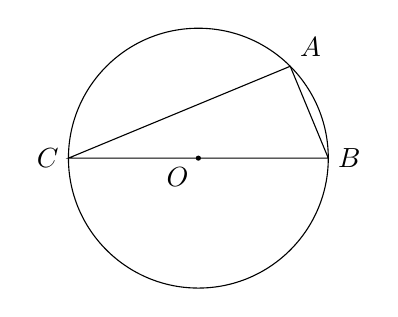
\begin{tikzpicture}[scale=0.55]
			          %projection ($(X)!(B')!(B)$)
			          %nommer chemin 'name path
			          %intersections \path [name intersections={of=d and gb,name=G}];
			          %intersection \path [name intersections={of=d and gb,by=G}];
			          %animation  \draw[visible on=<1>] 
				  %           \draw[visible on=<{2,4}>]
				  %angle arc[radius = 6mm, start angle= 180, end angle= 225] node [below left,pos=0.3]{$\alpha$}
				  %angle \pic [draw,"$\alpha$", angle eccentricity=1.5] {angle = A'--A--B};
				  %perpendiculaire ($(A')!3cm!-90:(A)$)
				  %cercle par point \node [draw] at (A) [circle through=(B)] {};
				  \coordinate[label=below left:$O$](O) at (0,0);
				  \coordinate[label=above right:$A$](A) at (45:3);
				  \coordinate[label=right:$B$](B) at (0:3);
				  \coordinate[label=left:$C$](C) at (-180:3);

				  \draw (O) circle (3cm);
				  \fill (O) circle (0.06);
				  \draw (A) -- (B) -- (C) -- cycle;				
				  \end{tikzpicture}
				  \end{figure}
				  Un triangle est inscrit dans un demi-cercle \textit{ssi} il est rectangle.
	 \column{.5\textwidth}    
				  \begin{figure}
				  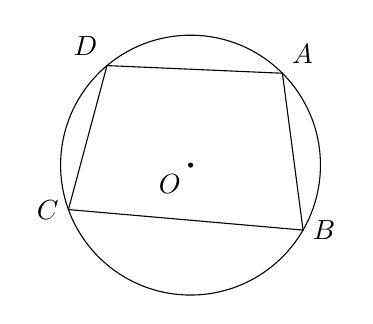
\begin{tikzpicture}[scale=0.55]
			          %projection ($(X)!(B')!(B)$)
			          %nommer chemin 'name path
			          %intersections \path [name intersections={of=d and gb,name=G}];
			          %intersection \path [name intersections={of=d and gb,by=G}];
			          %animation  \draw[visible on=<1>] 
				  %           \draw[visible on=<{2,4}>]
				  %angle arc[radius = 6mm, start angle= 180, end angle= 225] node [below left,pos=0.3]{$\alpha$}
				  %angle \pic [draw,"$\alpha$", angle eccentricity=1.5] {angle = A'--A--B};
				  %perpendiculaire ($(A')!3cm!-90:(A)$)
				  %cercle par point \node [draw] at (A) [circle through=(B)] {};
				  \coordinate[label=below left:$O$](O) at (0,0);
				  \coordinate[label=above right:$A$](A) at (45:3);
				  \coordinate[label=right:$B$](B) at (-30:3);
				  \coordinate[label=left:$C$](C) at (-160:3);
				  \coordinate[label=above left:$D$](D) at (130:3);

				  \draw (O) circle (3cm);
				  \fill (O) circle (0.06);
				  \draw (A) -- (B) -- (C) -- (D)-- cycle;				
				  \end{tikzpicture}
				  \end{figure}
				  Un quadrilatère convexe est inscrit dans un cercle \textit{ssi} ses angles opposés sont supplémentaires.
	\end{columns}
	\notedir{%
	.1 Figures inscrites.
	.2 Triangle inscrit dans demi-cercle est rectangle..
	.2 Quadrilatère inscrit dans cercle a angles opposés supplémentaires..
	}
}
\frame{ \frametitle{Cercles.} \underline{Cordes.} \\ \bigskip \centering
 \begin{figure}
				  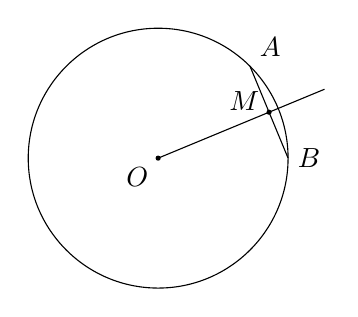
\begin{tikzpicture}[scale=0.55]
			          %projection ($(X)!(B')!(B)$)
			          %nommer chemin 'name path
			          %intersections \path [name intersections={of=d and gb,name=G}];
			          %intersection \path [name intersections={of=d and gb,by=G}];
			          %animation  \draw[visible on=<1>] 
				  %           \draw[visible on=<{2,4}>]
				  %angle arc[radius = 6mm, start angle= 180, end angle= 225] node [below left,pos=0.3]{$\alpha$}
				  %angle \pic [draw,"$\alpha$", angle eccentricity=1.5] {angle = A'--A--B};
				  %perpendiculaire ($(A')!3cm!-90:(A)$)
				  %cercle par point \node [draw] at (A) [circle through=(B)] {};
				  \coordinate[label=below left:$O$](O) at (0,0);
				  \coordinate[label=above right:$A$](A) at (45:3);
				  \coordinate[label=right:$B$](B) at (0:3);
				  \coordinate[label=above left:$M$,yshift=-1mm](M) at ($(A)!.5!(B)$);
				  \fill ($(A)!.5!(B)$) circle (0.06);
				  \draw (O) circle (3cm);
				  \fill (O) circle (0.06);
				  \draw (A) -- (B);
				  \draw (O) -- ($1.5*(A)!.5!(B)$);
				  \end{tikzpicture}
				  \end{figure}
				  La droite passant par le centre d'un cercle et le milieu d'une des cordes est perpendiculaire à cette corde.
				  
	\notedir{%
	.1 Médiatrice d'un corde.
	.2 Droite passant par centre et milieu corde est perpendiculaire à corde..
	}
}				
\end{document}

%%% Local Variables:
%%% mode: latex
%%% TeX-master: t
%%% End:
